\documentclass[12pt]{article}

\usepackage{mathrsfs}
\usepackage{epsfig}
\usepackage{graphicx}
\usepackage{color}
\usepackage{amsmath}
\usepackage{amsfonts}
\usepackage{amssymb}
\usepackage{amsthm}
\usepackage{amscd}
\usepackage{verbatim}
\usepackage{fullpage}
\usepackage{indentfirst}

%\setcounter{MaxMatrixCols}{20}
\theoremstyle{plain}
\newtheorem{theorem}{Theorem}[section]
\newtheorem{proposition}[theorem]{Proposition}
\newtheorem{lemma}[theorem]{Lemma}
\newtheorem{corollary}[theorem]{Corollary}
\newtheorem{conjecture}[theorem]{Conjecture}
\theoremstyle{definition}
\newtheorem{definition}[theorem]{Definition}
\newtheorem{notation}[theorem]{Notation}
\newtheorem{remark}[theorem]{Remark}
\newtheorem{example}[theorem]{Example}
\numberwithin{equation}{theorem}

\newcommand{\black}{\hfill{\ensuremath{\blacksquare}}}
\DeclareMathAlphabet{\mathpzc}{OT1}{pzc}{m}{it}

\graphicspath{ {./} }

\begin{document}
\begin{titlepage}
	\centering
	\vspace{4cm}
	{\scshape\Large DSE 220: Machine Learning\par}
	\vspace{1.5cm}
	{\huge\bfseries Final Project: Amazon Product Review\par}
	\vspace{2cm}
	{\Large\itshape Kevin Kannappan\par}

% Bottom of the page
	{\large \today\par}
\end{titlepage}


\section{Introduction}

Amazon is a leading e-commerce website and uses Macine Learning applications extensively in their products. Given Amazon data surrounding product reviews, our task was to predict how helpful the review will be - presumably, so that the predicted most helpful reviews are seen in order of decreasing helpfulness. The \textit{useful} information we were provided is as follows:
\begin{itemize}
\item \textbf{reviewText}: the written response of the review  (free-text)
\item \textbf{summary}: the headline of the review, theoretically the summary (free-text)
\item \textbf{price}: the price of the reviewed product (numeric)
\item \textbf{reviewTime}: the time of the review submission (string)
\item \textbf{category}: the provided category label of the reviewed product (numeric)
\item \textbf{categories}: more granular category labels of the reviewed product (lists of strings)
\item \textbf{rating}: the 1-5 star rating of the reviewed product (numeric)
\item \textbf{outOf}: the total number of votes the review received (dictionary: numeric)
\item \textbf{nHelpful}: \textit{target variable}, the number of votes that marked the review as ''Helpful" (dictionary: numeric)
\end{itemize}

\bigskip
The remainder of the data contained unique identifier values that would not be valuable for prediction. Some of my initial thoughts were that the \textit{summary} and \textit{reviewText} may have valuable information that could produce highly predictive features. Before that, however, we had to pre-process the data so that it could be developed into a training and test set.

\section{Data Pre-Processing}
\subsection{Initial Analysis}

Leveraging the notebook provided to us, we implemented the functions for reading and processing the data from its initial JSON (dictionary) format. The raw training and test data were both read into pandas dataframes where we previewed the data. The training data-set contained 200,000 rows and the test data-set contained 14,000 rows. Based on the amount of training data alone, simpler techniques such as kNN or Decision Trees were eliminated from contention as their performance on large data-sets is usually limited (computationally and predictive power) whereas deep-learning techniques could be considered as they have proven to be robust with large amounts of data. The target variable \textit{nHelpful} is continuous so we would implement a regression task as opposed to a classification one.

\bigskip
We also wanted to understand how complete or problematic our feature quality was. \textit{Null} or missing values can be especially challenging for models to overcome, depending on the data-type. Upon evaluating the distribution of \textit{null} values in the training set, we found that \textit{price} had missing values for $\approx$ 63\% of the training set. Considering that it is the majority of the data-set, we did not want to skew the feature by replacing the missing value with the mean price nor wanted to convert the feature into discrete values and giving it a missing label. Hence, \textit{price} was dropped from the training and test sets.

\subsection{Feature Engineering}

Abstracting back to the initial question at hand, can we predict the helpfulness of a review? When we think about modeling helpfulness, there are some initial things to consider. First, the product review (and concurrently helpfulness) is a product feature implemented by Amazon that is based on user behavior. Second, a review can only be marked as helpful if it is seen. Third, from experience, we know that particularly detailed or ''attention-grabbing" reviews happen to be the most helpful when we are searching for products. We knew that we had to model (or at least test) these three aspects in order for our predictions to be comprehensive:

\begin{itemize}
\item \textbf{Time}: the year or month of the review could be very important for a variety of reasons. First, since the feature review itself is a product that Amazon implemented on its platform, there may be ramp-up time until it was widely used by its members. Second, more recent reviews may contain less \textit{outOf} values and for a review to be helpful, it needs to be seen first. Third, there might be seasonality at-play when you consider the likelihood to mark a review as helpful (i.e. holiday season may see more helpful reviews as there is more pressure for shopping, etc.). Both the year and the month were extracted from the \textit{reviewTime} field using date manipulations and used as features.
\item \textbf{Flamboyance}: if the title of the review is especially ''eye-catching", then there is a good chance people will actually read the review. Hence, sentiment from the \textit{summary} field was developed as a feature. Specifically, the \textbf{vader sentiment} function from nltk was applied to the field and produced a normalize ''compound" sentiment score that produces a value between -1 (negative) and 1 (positive).
\item \textbf{Exhaustive}: based on experience, the more detailed the review, the more information received, thus the most informed decision can be made. It would be very difficult, not impossible, to scrape the \textit{reviewText} using NLP processing to gain some type of ''quality" review score. Something easier, would just be to take the word count in the review based on the assumption that the more words it contains, the more detail it has. The word count feature was extracted from the \textit{reviewText} field using string manipulation.
\end{itemize}

\bigskip
The final steps of the feature engineering process were to clean up the remaining features. All unique identifier features were dropped, and they were not mentioned above because they are not considered to be \textit{useful} features. \textit{categoryID} was converted into binary features using ''one-hot" encoding, as the numerical representation of the categories should not be used (i.e. can't make sense of the mean and standard deviation of clothing compared to tools). Lastly, the more specific \textit{categories} field was dropped because of the variance and lack of structure making it difficult to obtain usable information.

\section{Training Data Exploration}

Looking at the histogram distribution across the different features, we understood that the target variable had a fair amount of variability with some outlier values. This poses a significant problem for regression tasks as outliers are difficult to accurately predict. While one may discard the outlier values or reduce the dimensionality of the data-set in hopes of dealing with them, we figured that predicting outlier values would be important for this task (i.e. some items are highly rated). After initially attempting to model directly to \textit{nHelpful}, we realized that the results would contain too much error (detailed in subsequent section). Instead, we leveraged the fact that \textit{nHelpful} was a linear combination of \textit{outOf}. By effectively modeling the ratio between \textit{outOf} and \textit{nHelpful}, we dealt with the problem of outliers and provided an easier prediction space for the algorithms. The only adjustment that we would make is to multiply the new target ratio, \textit{helpful rate}, by the value of \textit{outOf} in the test set to provide the resulting predictions.

\bigskip
On the predictive features, we saw that \textit{categories} 2-4 were rarely present and for the most part had near zero variability. Considering we did not have many features to begin with, we left them in. Engineered features produced expected distributions and were likely to benefit the analysis. Since the interaction of the feature space is able to produce the model, we examined the covariance and correlation matrix. There were no real surprises with the results, depicted below:
\bigskip

\begin{figure}[!htb]
   \begin{minipage}{0.48\textwidth}
     \centering
     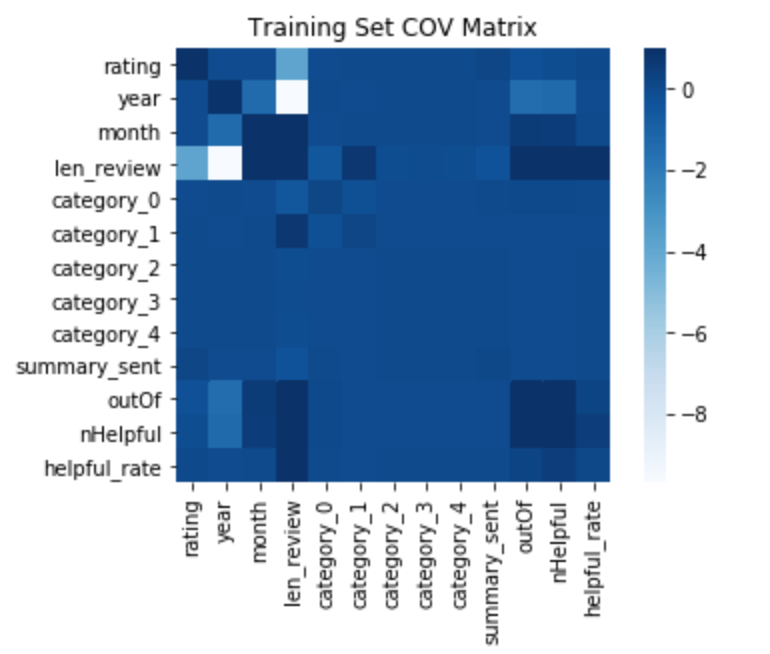
\includegraphics[width=.7\linewidth]{cov_matrix}
     \caption{Covariance Matrix of Features}\label{Fig: COV Matrix}
   \end{minipage}\hfill
   \begin{minipage}{0.48\textwidth}
     \centering
     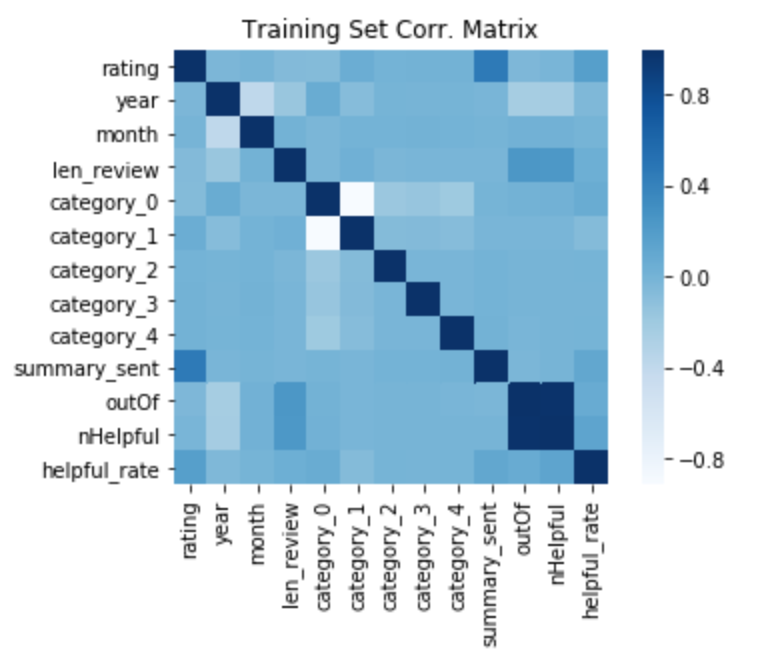
\includegraphics[width=.7\linewidth]{correlation_matrix}
     \caption{Correlation Matrix of Features}\label{Fig: Corr Matrix}
   \end{minipage}
\end{figure}
\bigskip
\bigskip

\section{Model Building}
\subsection{Method I: XGBoost Regressor on nHelpful}

Using the features outlined in the previous section, we first predicted the \textit{nHelpful} feature using Gradient Boosted Regression. Leveraging the base model (see attached code), we observed the plot of the boosted rounds on the training and validation \textbf{mean absolute error (mae)}. Depicted in the plot below, we recognized that the model was marginally outperforming the baseline prediction and we would need to tune the model further:

\bigskip
\begin{figure}[ht]
\begin{center}
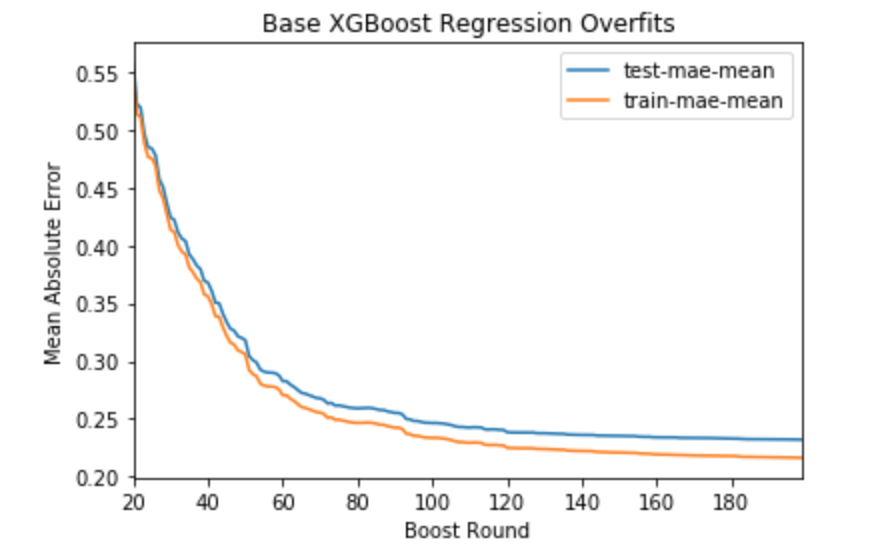
\includegraphics[width=10cm, height=6cm]{base_xgboost}
\caption{Initial Approach Proved Insightful}\label{Fig: XGboost Init}
\end{center}
\end{figure}

We implemented 5-fold cross-validation and used a grid search to tune the learning rate using the same default Gradient Boosted Regression model. The theory was that a slower learning rate would reduce the error and avoid over-fitting. Most of the time we were not doing better than the baseline prediction (mean MAE of 29). Based on the results and the subsequent feature importance graph, we realized that we were not going to get anywhere with this approach by predicting on such a large response distribution and decided to shift towards predicting on the ratio, \textit{helpful rate}.

\subsection{Method II: Ensemble Model: Classification \& Regression on Helpful Rate}

Our second approach involved predicting on the more structured \textit{helpful rate}, a linear combination of \textit{outOf} and \textit{nHelpful}. The task would be to then multiply the resulting prediction by the value for \textit{outOf} provided in the test set. Previously, when we examined the distribution of \textit{helpful rate}, we found some interesting insights. The value scaled from 0-1, which would make sense because it is a ratio, yet it was not normally distributed. Roughly 4\% of the data was exactly 0 (no helpful votes out of those chosen) and around 19\% of the data was exactly 1 (100\% helpful votes). With such a high distribution of binary outcomes, we decided to make the prediction an \textbf{ensemble} of models. More specifically, for training set values $\in \{0,1\}$, build a Gradient Boost Classifier (or Logistic Regression), else build a Gradient Boost Regression. The idea for this development follows many Kaggle competitions where an aggregation of models, specifically better suited to certain tasks, provide better overall predictions. In this case, we did not want any error for those that are 0 or 1 outcomes, and we want to maximize our predictive accuracy on those values.

\bigskip
By leveraging two models, we are able to gather different feature interactions for each use case and should provide more robust results. For the classification component, perhaps certain features are more relevant to predicting whether or not a single vote will be helpful whereas in the case of a review that gets more traction, there might be other factors that might be more important in predicting the ratio of helpful reviews. Looking at the importance graphs below, we found that this was the case as the respective models fit to their subset training set: 

\begin{figure}[!htb]
   \begin{minipage}{0.48\textwidth}
     \centering
     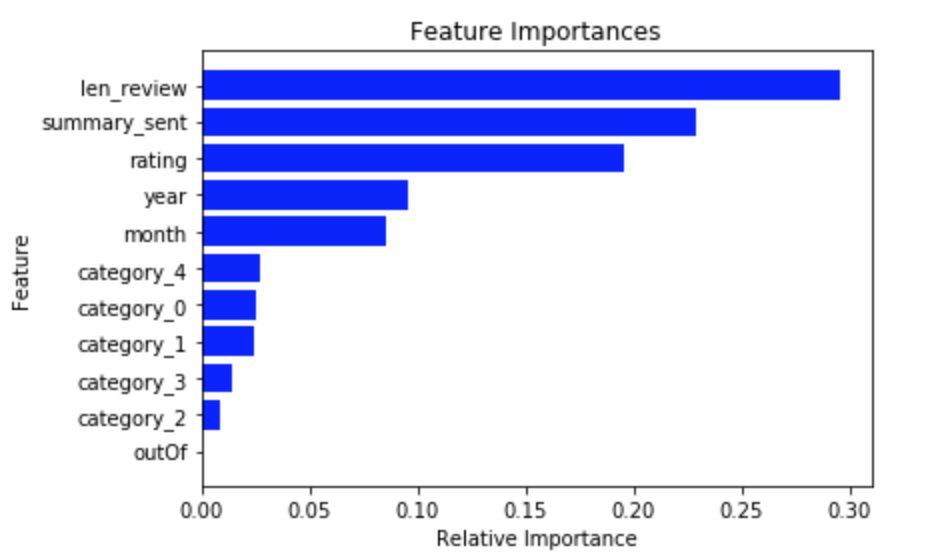
\includegraphics[width=1.1\linewidth]{xgb_class}
     \caption{Gradient Boost Classification}\label{Fig: Class Feature Importance}
   \end{minipage}\hfill
   \begin{minipage}{0.48\textwidth}
     \centering
     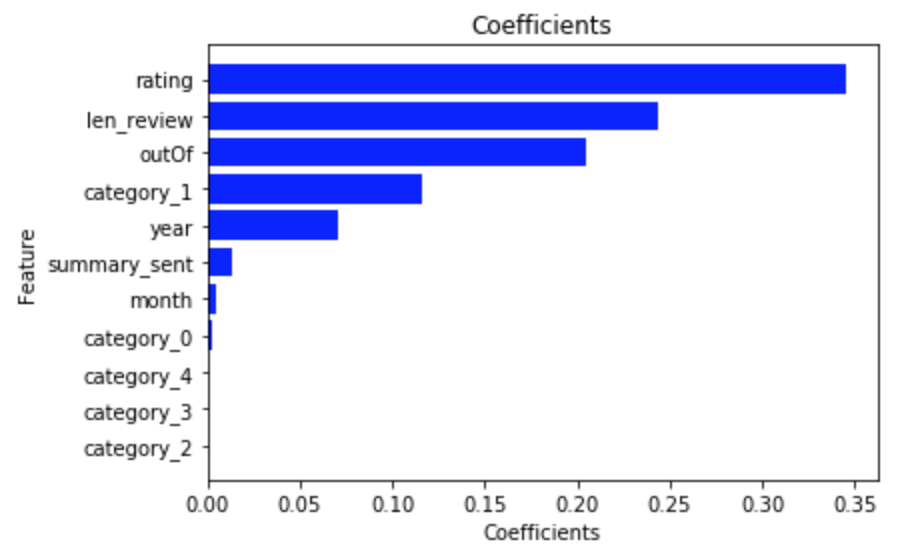
\includegraphics[width=1.1\linewidth]{xgb_regress}
     \caption{Gradient Boost Regression}\label{Fig: Reg Feature Importance}
   \end{minipage}
\end{figure}
\bigskip

\bigskip
The final model(s) used in our second method involved the following approach: iteratively create random training and validation sets, in 5-fold cross-validation to be tuned in a grid search. We used 2 classification models for the binary classification portion: Logistic Regression and Gradient Boost Classifier where we tuned the former on cost and regulariziation technique and the latter on learning rate and loss function. For the regression training data, we used a Gradient Boosting Regression in both cases and also tuned the learning rate and loss function. 

\bigskip
Upon final analysis, we found both techniques in Method II to be robust and predict well in validation ($\approx$ 16.7 MAE). We submitted both techniques to Kaggle and both well outperformed the thresholds for assessment on the public portion of the data. The final approach of iteratively creating new training and validation sets was a successful approach for finding a successful model that generalizes well. We will use this technique in future research.

\end{document}